\documentclass[../main.tex]{subfiles}

\begin{document}
\section{Resumo ideia}
\begin{figure}[H]
\centering
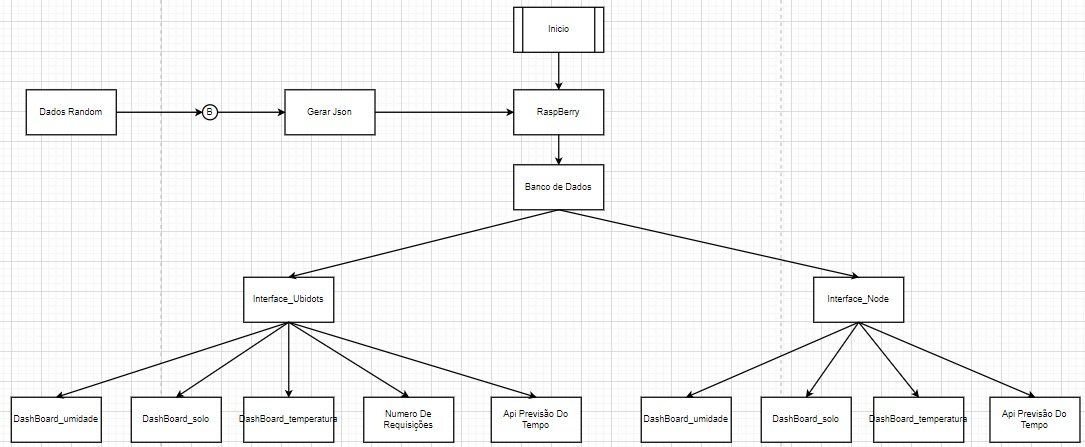
\includegraphics[scale=0.35]{../../UML image.jpeg}
\end{figure}

A ideia inicial é para gerar um sistema de monitoramento que fica rastreando o desenvolvimento de plantas que o usuário possa estar cultivando no momento. \newline
O projeto será composto de módulos visuais, temperatura e umidade para analisar os detalhes da terra, combinado com um webpage e notificações ao usuário baseado em necessidades. \newline

\end{document}